% !TEX TS-program = pdflatex
% !TEX encoding = UTF-8 Unicode

% This is a simple template for a LaTeX document using the "article" class.
% See "book", "report", "letter" for other types of document.

\documentclass[11pt]{article} % use larger type; default would be 10pt

\usepackage[utf8]{inputenc} % set input encoding (not needed with XeLaTeX)

%%% Examples of Article customizations
% These packages are optional, depending whether you want the features they provide.
% See the LaTeX Companion or other references for full information.

%%% PAGE DIMENSIONS
\usepackage{geometry} % to change the page dimensions
\geometry{a4paper} % or letterpaper (US) or a5paper or....
% \geometry{margin=2in} % for example, change the margins to 2 inches all round
% \geometry{landscape} % set up the page for landscape
%   read geometry.pdf for detailed page layout information

\usepackage{graphicx} % support the \includegraphics command and options

% \usepackage[parfill]{parskip} % Activate to begin paragraphs with an empty line rather than an indent

%%% PACKAGES
\usepackage{tikz}
\usepackage{booktabs} % for much better looking tables
\usepackage{color} % Added by me
\usepackage{array} % for better arrays (eg matrices) in maths
\usepackage{paralist} % very flexible & customisable lists (eg. enumerate/itemize, etc.)
\usepackage{verbatim} % adds environment for commenting out blocks of text & for better verbatim
\usepackage{subfig} % make it possible to include more than one captioned figure/table in a single float
% These packages are all incorporated in the memoir class to one degree or another...

%%% HEADERS & FOOTERS
\usepackage{fancyhdr} % This should be set AFTER setting up the page geometry
\pagestyle{fancy} % options: empty , plain , fancy
\renewcommand{\headrulewidth}{0pt} % customise the layout...
\lhead{}\chead{}\rhead{}
\lfoot{}\cfoot{\thepage}\rfoot{}

%%% SECTION TITLE APPEARANCE
\usepackage{sectsty}
\allsectionsfont{\sffamily\mdseries\upshape} % (See the fntguide.pdf for font help)
% (This matches ConTeXt defaults)

%%% ToC (table of contents) APPEARANCE
\usepackage[nottoc,notlof,notlot]{tocbibind} % Put the bibliography in the ToC
\usepackage[titles,subfigure]{tocloft} % Alter the style of the Table of Contents
\renewcommand{\cftsecfont}{\rmfamily\mdseries\upshape}
\renewcommand{\cftsecpagefont}{\rmfamily\mdseries\upshape} % No bold!

%%% END Article customizations

%%% The "real" document content comes below... %%%

\title{Combinations}
\author{Ethan Schaffer}
\date{Due 11/1/16}
\newcommand\tab[1][1cm]{\hspace*{#1}}

\begin{document}
\maketitle
\section* {Problem}
\textit{How many ways can 10 children be arranged in a circle? (Two arrangements are different if some child has a different child either on the right or on the left.)}

\section*{Solution}
I conclude that ten children can be arranged in a circle \textbf{9!} different ways. To solve this problem, I looked to what I already knew about permutations. To solve this problem, I realized that a different way to express the problem is: 
\\ \textit{How many ways can 9 children be arranged in relation to one child?}
\\ \tab My reasoning for this is that no matter where in a circle the tenth child is, the circle's identity can only be changed when two children switch places. For example, the two circles below are the same.
\\
\\
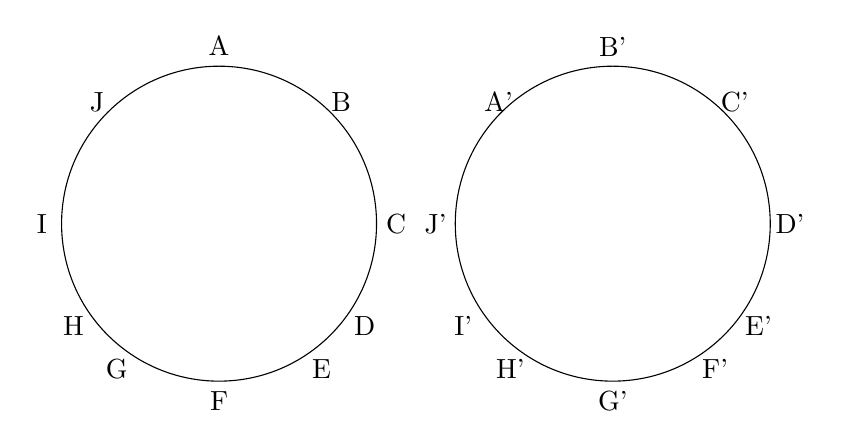
\begin{tikzpicture}
\draw (0,0) circle (2cm);
\draw (0,2.25) node {A}; \draw (1.55, 1.55) node {B};
\draw (2.25, 0) node {C}; \draw (1.85, -1.3) node {D};
\draw (1.3, -1.85) node {E}; \draw (0, -2.25) node {F};
\draw (-1.3, -1.85) node {G}; \draw (-1.85, -1.3) node {H};
\draw (-2.25, 0) node {I}; \draw (-1.55, 1.55) node {J};

\draw (5,0) circle (2cm);
\draw (5,2.25) node {B'}; \draw (6.55, 1.55) node {C'};
\draw (7.25, 0) node {D'};\draw (6.85, -1.3) node {E'};
\draw (6.3, -1.85) node {F'}; \draw (5, -2.25) node {G'};
\draw (3.7, -1.85) node {H'}; \draw (3.1, -1.3) node {I'};
\draw (2.75, 0) node {J'}; \draw (3.55, 1.55) node {A'};
\end{tikzpicture}
\\ Based on how these circles are the same, I knew that my solution must be smaller than 10!. There is no difference, after all, between these two circles. To prove this, I looked at the relationship between where each child (represented by a letter) is in relation to child A (or A'). Based on this reasoning,  I decided that I could redraw the circle as
\\
\\
\begin{tikzpicture}
\draw (0,0) circle (2cm);
\draw (0,2.25) node {A}; \draw (1.55, 1.55) node {9};
\draw (2.25, 0) node {8}; \draw (1.85, -1.3) node {7};
\draw (1.3, -1.85) node {6}; \draw (0, -2.25) node {5};
\draw (-1.3, -1.85) node {4}; \draw (-1.85, -1.3) node {3};
\draw (-2.25, 0) node {2}; \draw (-1.55, 1.55) node {1};
\end{tikzpicture}
\\ \tab
where A is a `starting' child and each number represents how many children are left to choose from. As such, I have converted the combinations problem into a permutations problem. As we have already proven, when finding permutions of n objects arrranged one at a time in any order, the number of permutations is n!. Based on this, I was able to conclude that the solution is \textbf{9!}. 
\\  \tab An interesting observation I made is that every circle can be redrawn (via rotation) ten different ways. If we count each of those rotations as its own circle, we would have 10! possible circles. This relates to combinations in that by changing our ruling on unique circles, we actually turned the problem into a question of permutations. 

\section* {Analysis}
\tab This problem was very interesting. I am curious if we will find a more broad formula. It seems like Alex's formula ($\frac{n!}{k!(n-k)!}$) might useful for combinations, but I am not 100\% sure how to apply it. 

\section* {Status}
\tab I feel like I fully understand this problem.

\section* {MVP}
\tab My MVPs for this problem are Matthew and Teles. They were the ones I talked about this problem with, and I gained a deeper understanding of the problem through explaining my solution to them.
\end{document}
